% ------------------------------------------------------------------------------
% Introduce the topic - What characterizes the topic?
% Introduce the goal - What do you want to achieve with your thesis?
% Make the reader curious - What motivates the reader to read on?
% Describe the relevance - Why is this bachelor thesis scientifically relevant?
%
% The introduction should have the following content:
% - Initial situation & presentation of the topic - You introduce the topic with an exciting 'bait'. You provide initial information on the topic and the object of research and explain the current state of research.
% - Relevance of the topic & motivation - You justify the relevance of your topic (scientifically) and place it in the context of your field. In addition, it is often required that you disclose your personal motivation.
% - Problem description and thematic delimitation - By means of a specific research question (or hypothesis) you present your explicit research interest. If necessary, explain technical terms.
% - Objectives - Your introduction should clearly state what the goal of your paper is and what outcome you hope to achieve upon completion of the bachelor thesis.
% - Method You explain the approach and justify the choice of method.
% - Structure of the Bachelor's thesis - Finally, you give the reader a general overview of your Bachelor's thesis by explaining the structure, showing the red thread and how the research question is answered.
% ------------------------------------------------------------------------------

\opt{never}{\addbibresource{03-tail/bibliography.bib}} % to make citation found in most IDE

\chapter{Introduction}
\label{chap:introduction}

% -- Your text goes here --
For a long time, embedded systems remained isolated from each other. Now it's time to bring them together with the world of the \gls{cloud}. Hardware devices have always been limited in terms of resources. Designs have allowed them to evolve according to their use case. However, physical limits have been observed. This is how the \hyperref[subsec:cloudcomputing]{cloud computing} came into being, partly in response to these difficulties.

The \gls{cloud} provides a huge number of advantages. It frees up hardware resources to optimise the operation of embedded systems. It is likely that these systems will not be able to perform complex calculations. The \hyperref[subsec:cloudcomputing]{cloud computing} has the capacity to do this. The storage problem is another constraint. The \hyperref[subsec:cloudcomputing]{cloud computing} offers almost unlimited storage. It doesn't stop there. It is capable of offering constant scalability to infrastructures. It is made up of different independent services that can be easily connected together. There is vertical scaling, which means increasing the size of a resource, and horizontal scaling, which means increasing the number of resources.

More and more engineers have decided to take an interest in this area in order to interconnect their embedded systems with the \gls{cloud}. This practice is an integral part of the \nameref{subsec:iot}. Due to increasingly large projects, not to mention artificial intelligence, they want to use \hyperref[subsec:cloudcomputing]{cloud computing} environments in order to no longer be constrained by resources. To make it easier to use a \gls{cloud_infrastructure}, companies have decided to offer \gls{cloud} platforms comprising a multitude of services for all types of use (\gls{aws}, Microsoft Azure, etc). It's also a way of letting engineers work on their business rather than worrying about maintaining and securing these infrastructures.


% -----------------------------------------------------------------------------
\section{56K.\Gls{cloud}}
\label{subsec:56k.cloud}

% -- Your text goes here --
\nameref{subsec:56k.cloud} is a company based in Sion (Valais) since 2018. It offers various services through the \gls{cloud}. It provides solutions for businesses that want to improve their processes while reducing their costs. It is also a consultancy firm that seeks to promote the \gls{cloud} to customers who find it difficult to understand certain concepts in this rapidly expanding digital world. Collaborations with a number of partners are also an asset, enabling us to pool a wide range of skills to provide customers with a complete product. In order to share its vision of the \gls{cloud} more widely, it has additional premises in Winterthur (Zurich).
\begin{center}
    \begingroup
    
\includegraphics[width=0.5\columnwidth]{introduction/enterprise_logo.png}
    \captionof{figure}{\nameref{subsec:56k.cloud} company logo \cite{enterprise_56k.cloud}}
    \label{fig:enterprise_logo}
    \endgroup
\end{center}
The idea of a \gls{cloud} solution is to move an on-premise infrastructure to the \gls{cloud}. It's a way of reducing costs by only paying for what you use (pay-as-you-go), and by having something that can be easily scalable. It's also a good way of increasing the speed of processes by using optimal resources for each application.

In terms of consultancy, \nameref{subsec:56k.cloud} introduces \nameref{subsec:cloudnative} technology to customers who want to find out more. It also covers the subject of \acrshort{devops} and containerisation.


% -----------------------------------------------------------------------------
\section{Problem}

% -- Your text goes here --
While \nameref{subsec:56k.cloud} mainly offers \gls{cloud} solutions, this company also works in the \acrfull{iot} sector. Recently, it quickly noticed a major problem between embedded systems engineers and those from the world of \gls{cloud}. More and more engineers are asking for devices to be able to link easily and quickly to a \gls{cloud_infrastructure}. However, there is currently no reference architecture that enables an infrastructure to be deployed and an embedded system to be provisioned directly.

This is a real problem because of the time needed and the difficulty for engineers to link hardware to a \gls{cloud_infrastructure}. Because of the two distinct professions, a person coming from the \gls{cloud} will need time to understand and set up an operating system capable of connecting to an infrastructure. And vice-versa, a person coming from the hardware world will need to familiarise themselves with a \gls{cloud_infrastructure}, not to mention setting it up while using the best practices of the \nameref{subsec:cloudnative}.
\begin{center}
    \begingroup
    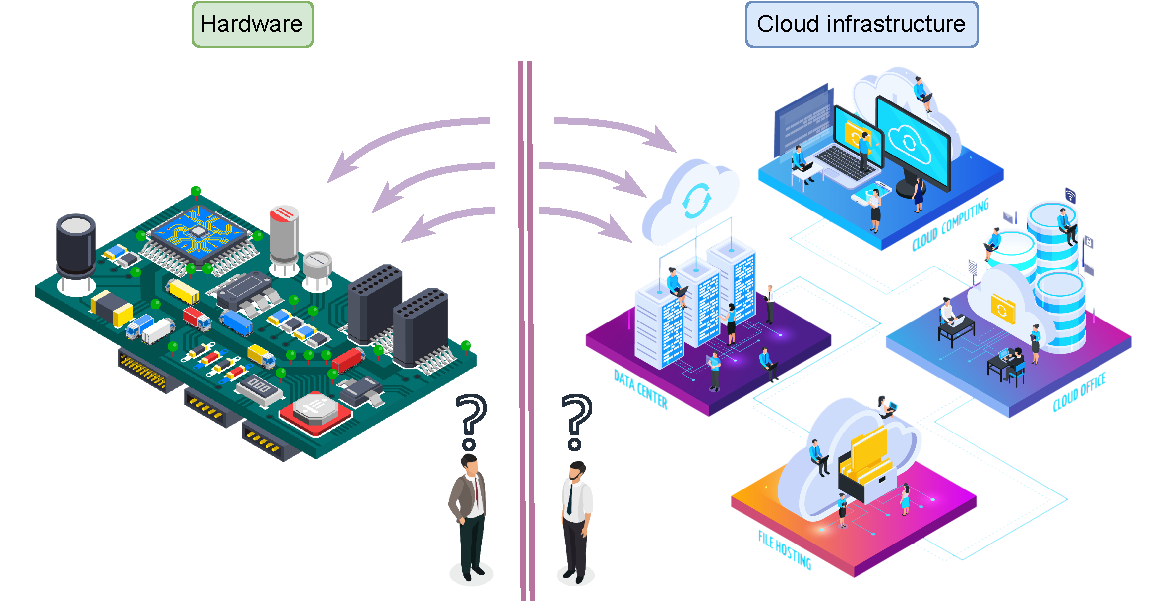
\includegraphics[width=1\columnwidth]{introduction/problem.pdf}
    \captionof{figure}{The problem of linking the hardware to the \gls{cloud_infrastructure} \cite{images_freepik}}
    \label{fig:problem}
    \endgroup
\end{center}
The need to find a solution arose when engineers started asking electronic board manufacturers to design equipment offering services for linking to a \gls{cloud_infrastructure}. Since these manufacturers are not in this discipline, they do not want to spend time developing these types of solutions. It is therefore possible to identify the main players affected. There are the hardware engineers who are unable to meet the new needs of customers. Cloud engineers, who want to do the job for them, have to devote part of their time to introducing embedded concepts. Learning something new can quickly become time-consuming.

Nevertheless, a few solutions are gradually emerging. However, these remain very closed. There is no open source reference architecture capable of satisfying a wide range of products. These solutions therefore remain highly proprietary.


% -----------------------------------------------------------------------------
\section{Objectives}

% -- Your text goes here --
The primary aim of this work is to develop a reference architecture enabling the deployment of a \gls{cloud_infrastructure} with the \gls{provisioning} of a fleet of embedded systems. The idea is to be able to automatically provision devices to the infrastructure when they are first started up. The infrastructure must contain the essential minimum of components to make the architecture as universal as possible. Since \nameref{subsec:56k.cloud} is a partner of \gls{arm}, a processor manufacturer, the embedded systems must be equipped with this. It should be added that \gls{arm} puts certifications on their components such as SystemReady. SysteamReady program guarantees that an operating system and the following software layers can function correctly in their processors. The embedded systems used in this project must be certified SystemReady. In addition, the infrastructure must be deployed on the \gls{aws} platform. This is the \gls{cloud} provider that \nameref{subsec:56k.cloud} works with.
\begin{center}
    \begingroup
    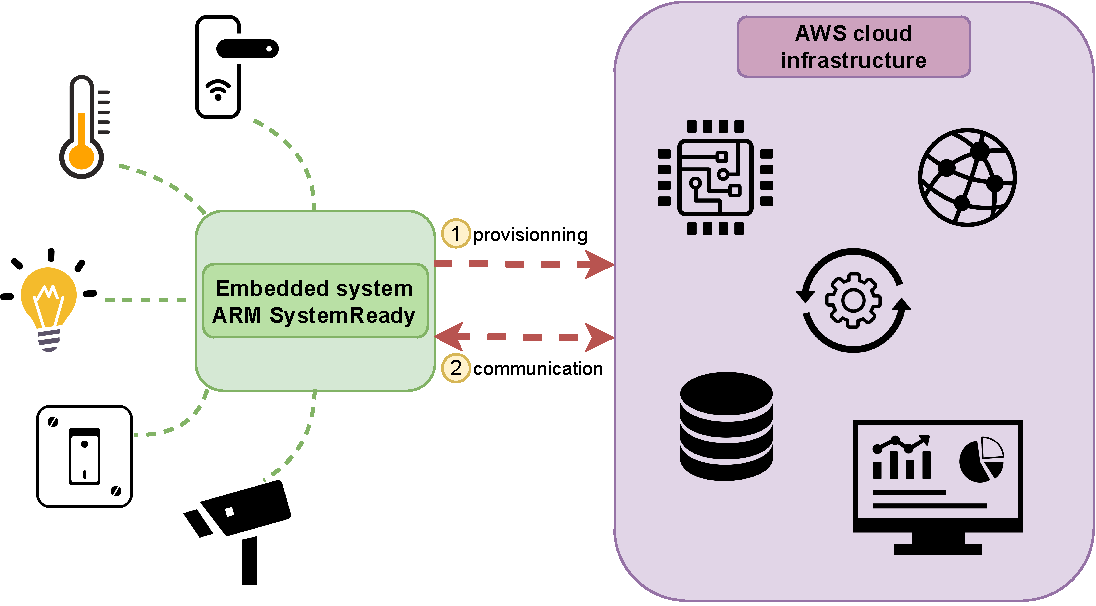
\includegraphics[width=1\columnwidth]{introduction/objective.pdf}
    \captionof{figure}{Overview of objectives}
    \label{fig:objective}
    \endgroup
\end{center}
The aim of this project is to be open source so that a community can form around it. It should enable embedded systems and \gls{cloud} engineers to use this reference architecture easily. They need to be able to focus on their final product. The best practices of \nameref{subsec:cloudnative} must be used for the development of this project. In order to guarantee a sound architecture, the use of \acrfull{ci} and \acrfull{cd} tools are essential. In addition, to ensure compatibility, the architecture must be functional on different embedded systems with a \gls{arm} processor and certified SystemReady.

Secondly, once the reference architecture is functional, a demonstration project must be based on it. This is a proof of concept. The general idea is to deploy a \gls{cloud_infrastructure} on \gls{aws} and have various \gls{cloud} services automatically set up to interact with the embedded system. Data will then transit between these two worlds and it must be viewable from an interface.


% -----------------------------------------------------------------------------
\section{Project plan}

% -- Your text goes here --
Figure \ref{fig:work_packages} shows the project plan in the form of \glspl{work_package}.
\begin{center}
    \begingroup
    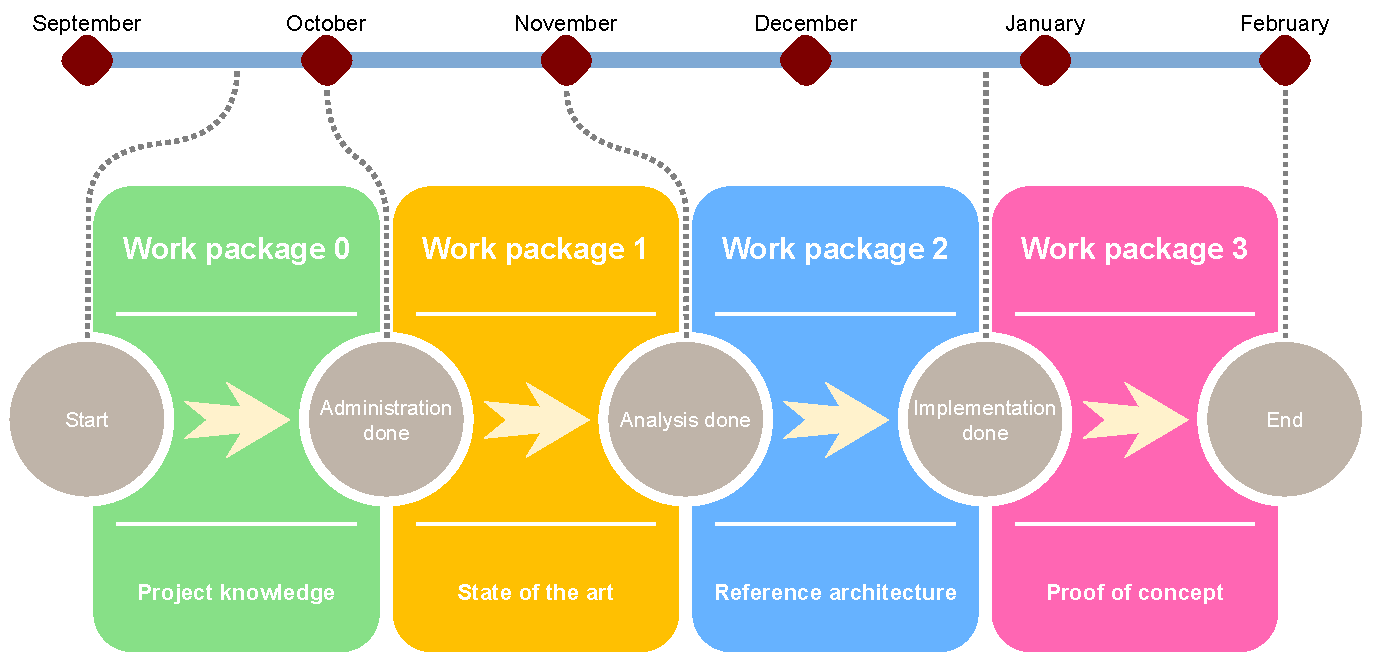
\includegraphics[width=1\columnwidth]{introduction/work_packages.pdf}
    \captionof{figure}{Project plan}
    \label{fig:work_packages}
    \endgroup
\end{center}
The first \gls{work_package} contains all the administration. It involves learning about the project, being aware of the issues and clearly defining the specifications. This takes around two weeks.

About a month is spent researching existing solutions that are closest to the project. This involves drawing up a state of the art by researching scientific articles and other documentation.

The third \gls{work_package} concerns the reference architecture. Almost two months are devoted to this. This implementation part will be the final product, which will be delivered as open source on a shared repository.

In order to validate this architecture, a proof of concept will be carried out. This is the final \gls{work_package}. It will take just over a month. Tests will be carried out to prove that it works properly.

% -----------------------------------------------------------------------------
\section{Research methodology}

% -- Your text goes here --
The research methodology used in this thesis was first to draw up a state of the art on existing solutions that are as close as possible to this project. An overview of the reference architecture was then drawn up with a view to implementing it more easily. A choice of development tools was also made. At the same time, the implementation was designed. Finally, the results were validated by means of a proof of concept.

The agile methodology, known as \gls{scrum}, was used throughout the project. It allows for iterative project management. Weekly meetings were arranged with the professor in charge of the project and, optionally, with some of the company's staff. To enable the project to progress efficiently, the \gls{kanban} method was used. This consists of virtual cards, each referring to a task. These cards are categorised in a table to determine the progress of each task. It's also a way of dividing the project into smaller parts so that time can be better estimated over the course of the project.


% -----------------------------------------------------------------------------
\section{Structure of this report}

% -- Your text goes here --
The \ref{chap:methodology} chapter (\nameref{chap:methodology}) contains a number of project methodologies for effective project management. The tools used are also described in addition to the training provided.

The \ref{chap:analysis} chapter (\nameref{chap:analysis}) contains several definitions and the state of the art. These are definitions of important terms that make up the project. The state of the art concerns the existing solutions that are closest to this project.

The \ref{chap:design} chapter (\nameref{chap:design}) contains an overview of the entire reference architecture. It includes the \gls{cloud_infrastructure}, the integration of embedded systems, the \acrshort{ci}/\acrshort{cd} pipeline and the applications.

The \ref{chap:implementation} chapter (\nameref{chap:implementation}) contains the implementation of all the parts included in the reference architecture. The tools used and how they work are presented.

The \ref{chap:validation} chapter (\nameref{chap:validation}) contains the analysis and validation of the results of the reference architecture.

The \ref{chap:conclusions} chapter (\nameref{chap:conclusions}) concludes the thesis by outlining the current state of the research, the problems encountered and future steps.